\chapter{Finite State Machines\label{chapter:finit-state-machines.tex}} 
In the previous chapter we have seen how to generate a scanner using \textsc{Ply}.  In this chapter
we learn how regular expressions can be implemented using \blue{finite state machines},
abbreviated as \textsc{Fsm}s.  There are two kinds of \textsc{Fsm}s: The deterministic ones and
non-deterministic ones.  Although non-deterministic \textsc{Fsm}s seem to be more powerful than
deterministic \textsc{Fsm}s, we will see that every non-deterministic \textsc{Fsm} can be transformed
into an equivalent deterministic \textsc{Fsm}.  After proving this result, we show how a regular
expression can be translated into an equivalent non-deterministic \textsc{Fsm}.  Finally, we show that the
language recognized by any \textsc{Fsm} can be described by an equivalent regular expression.  Therefore, the
central result of this chapter is the equivalence of finite state machines and regular expressions.
Hence, the results proved in this chapter are as follows:
\begin{enumerate}
\item The language described by a regular expression can be defined by a non-deterministic \textsc{Fsm}.
\item Every non-deterministic \textsc{Fsm} can be transformed into an equivalent deterministic \textsc{Fsm}.
\item For every deterministic \textsc{Fsm} there is an regular expression specifying the language recognized by
      the \textsc{Fsm}.
\end{enumerate}


\section{Deterministic Finite State Machines}
The \textsc{Fsm}s that we are going to discuss in this chapter are used to read a string and
to decide whether this string is an element of a given language.  Hence, the input of these 
\textsc{Fsm}s is a string, while the output is either the value \texttt{True} or the value \texttt{False}.
The name giving feature of an \textsc{Fsm} is the fact that an \textsc{Fsm} only has a
\underline{finite} number of possible states.  Reading a character causes the \textsc{Fsm} to change its state.
An \textsc{Fsm} accepts its input if it has reached a so called \blue{accepting state} after reading
all characters of the input string.  Let me explain this idea more precisely:
\begin{enumerate}
\item Initialy, the \textsc{Fsm} is in a state that is know as the \blue{start state}. \index{start state}
\item In every step of its computation, the \textsc{Fsm} reads one character of the input string
      $s$.  Every time a character is processed, the state of the \textsc{Fsm} might change.
\item Some states of the \textsc{Fsm} are designated as \blue{accepting states}.  \index{accepting state}
      If the \textsc{Fsm} has consumed all characters of the given input string $s$ and the \textsc{Fsm}
      has reached an accepting state, then the input string $s$ is accepted and the \textsc{Fsm}
      returns \texttt{True}.  Otherwise the \textsc{Fsm} returns \texttt{False} and the string $s$
      is rejected.
\end{enumerate}
\begin{figure}[!ht]
  \centering
      \epsfig{file=Abbildungen/abstara.eps, scale=0.7}
   \caption{An \textsc{Fsm} to recognize the language $L(\texttt{a}^*\cdot\texttt{b}\cdot\texttt{a}^*)$.}
  \label{fig:abstara.dot}
\end{figure}


\noindent
Finite state machines are best presented graphically.  Figure \ref{fig:abstara.dot} depicts a simple
\textsc{Fsm} that recognizes those strings that are specified by the regular expression
\\[0.2cm]
\hspace*{1.3cm}
$\texttt{a}^*\cdot\texttt{b}\cdot\texttt{a}^*$.
\\[0.2cm]
This \textsc{Fsm} has but two states.  These states are called $0$ and $1$.
\begin{enumerate}
\item State $0$  is the start state.  In Figure \ref{fig:abstara.dot}, the start state is indicated by an arrow
      comming from nowhere that points to it.  
  
      If the \textsc{Fsm} is in the state 0 and reads the character ``\texttt{a}'', then the
      \textsc{Fsm} stays in the state 0.  This is specified in the figure by an arrow labeled with the
      character ``\texttt{a}'' that both starts and ends in the state 0.  On the other hand, if the
      character ``\texttt{b}'' is read while the \textsc{Fsm} is in state 0, then the \textsc{Fsm}
      switches into the state 1.  This is depicted by an arrow labeled with the character
      ``\texttt{b}'' that originates from the state 0 and points to the state 1.
\item State  $1$ is an accepting state. In Figure \ref{fig:abstara.dot} this is specified by the
      fact that the state 1 is decorated by a double circle.

      If the character ``\texttt{a}'' is read while the \textsc{Fsm} is in state 1, then the
      \textsc{Fsm} does not change its state.  On the other hand, if the \textsc{Fsm} reads the
      character ``\texttt{b}'' while in state 1, then the next state is undefined since there is no
      arrow originating from state 1 that is labeled with the character ``\texttt{b}''.

      In general, a \textsc{Fsm} \blue{dies} \index{death of an \textsc{Fsm}}
      if it reads a character $c$ in a state $s$ such that there is no transition from $s$ when $c$ is read.
      In this case, the \textsc{Fsm} returns the value \texttt{False} to signal that it does not accept the given
      input string.
\end{enumerate}

\noindent
Formally, a \href{http://en.wikipedia.org/wiki/Finite-state_machine}{\emph{finite state machine}} 
\index{finite state machine}
is defined as a 5-tuple.
\begin{Definition}[\textsc{Fsm}]
A \blue{finite state machine} (abbreviated as \textsc{Fsm}\index{\textsc{Fsm}}) is a 5-tuple 
\\[0.2cm]
\hspace*{1.3cm}
$F = \langle Q, \Sigma, \delta, q_0, A\rangle$
\\[0.2cm]
where the components $Q$, $\Sigma$, $\delta$, $q_0$, and $A$ have the following properties:
\begin{enumerate}
\item $Q$ is the \underline{finite} \blue{set of states}.
\item $\Sigma$ is the \blue{input alphabet}\index{input alphabet}\index{$\Sigma$}.  Therefore, $\Sigma$ is a
      set of characters and 
      the strings read by the \textsc{Fsm} $F$ are strings from the set $\Sigma^*$.
\item $\delta: Q \times \Sigma \rightarrow Q \cup \{ \Omega \}$

      is the  \blue{transition function}\index{transition function}.  For every state $q\in Q$ and for all
      characters $c \in \Sigma$ the expression $\delta(q,c)$ computes the new state of the \textsc{Fsm} $F$
      that is reached if $F$ reads the character $c$ while in state $q$.
      If $\delta(q,c) = \Omega$, then $F$ \blue{dies} when it is in state $q$ and the next character
      is $c$. 

      In the figures depicting \textsc{Fsm}s transitions of the form $\delta(q, c) = \Omega$ 
      are not shown.
\item $q_0 \in Q$ is the \blue{start state}. \index{start state}
\item $A \subseteq Q$ is the set of \blue{accepting states}. \index{accepting states, set of}
      \qed
\end{enumerate}
\end{Definition}

\exampleEng
The \textsc{Fsm} that is shown in Figure  \ref{fig:abstara.dot} is formally defined as follows:
\\[0.2cm]
\hspace*{1.3cm}
$F = \langle Q, \Sigma, \delta, q_0, A \rangle$,
\\[0.2cm]
where we have:
\begin{enumerate}
\item $Q = \{ 0, 1 \}$,
\item $\Sigma = \{ \texttt{a}, \texttt{b} \}$,
\item $\delta = \bigl\{ 
                        \pair(0,a) \mapsto 0, 
                        \pair(0,b) \mapsto 1, 
                        \pair(1,a) \mapsto 1, 
                        \pair(1,b) \mapsto \Omega 
                \bigr\}$,
\item $q_0 = 0$,
\item $A = \{ 1 \}$.
\end{enumerate}
In order to formally define the language $L(F)$ that is accepted by an \textsc{Fsm} $F$
we generalize the transition function $\delta$ to a new function
\\[0.2cm]
\hspace*{1.3cm}
$\delta^*: Q \times \Sigma^* \rightarrow Q \cup \{ \Omega \}$
\\[0.2cm]
that, instead of a single character, accepts a string as its second argument.  The definition of
$\delta^*(q, w)$ is given by induction on the string $w$.
\begin{enumerate}
\item[I.A.] $w = \varepsilon$:  We define
            \\[0.2cm]
            \hspace*{1.3cm}
            $\delta^*(q, \varepsilon) := q$,
            \\[0.2cm]
            because if a deterministic \textsc{Fsm} does not read any character, it cannot change its state. 
\item[I.S.] $w = cv$ where $c \in \Sigma$ and $v  \in \Sigma^*$:  We define
            \\[0.2cm]
            \hspace*{1.3cm}
            $\delta^*(q, cv) := \left\{
            \begin{array}[c]{ll}              
            \delta^*\bigl(\delta(q,c),v\bigr) & \mbox{provided $\delta(q,c) \not= \Omega$;} \\
            \Omega                            & \mbox{otherwise}.
            \end{array}
            \right.
            $
            \\[0.2cm]
            If $F$ reads the string  $cv$, it first reads the character $c$.  Now if this causes  $F$
            to change into the state $\delta(q,c)$, then $F$ has to read the string $v$ in the state
            $\delta(q,c)$.  However, 
            if  $\delta(q,c)$ is undefined, then  $\delta^*(q,cv)$ is undefined too.
\end{enumerate}

\begin{Definition}[Accepted Language, $L(F)$]
  \index{accepted language} \index{$L(F)$}
  For an \textsc{Fsm} $F = \langle Q, \Sigma, \delta, q_0, A \rangle$ the \blue{language accepted by $F$} 
  is called $L(F)$ and is defined as
  \\[0.2cm]
  \hspace*{1.3cm}
  $L(F) := \bigl\{ s \in \Sigma^* \mid \delta^*(q_0,s) \in A \bigr\}$. 
  \\[0.2cm]
  Hence, the accepted language of $F$ is the set of all those strings that take $F$ from its
  start state into an accepting state. \eox
\end{Definition}

\exerciseEng
Specify an \textsc{Fsm} $F$ such that $L(F)$ is the set of all those strings $s \in \{a,b\}^*$, 
such that $s$ contains the substring  ``\texttt{aba}''.
\eox


\paragraph{Complete Finite State Machines}
Occasionally it is beneficial for an \textsc{Fsm} $F$ to be \blue{complete}: An \textsc{Fsm}
\\[0.2cm]
\hspace*{1.3cm}
$F = \langle Q, \Sigma, \delta, q_0, A \rangle$,
\\[0.2cm]
is \blue{complete}\index{complete, finite state machine} if the transition function $\delta$ never returns the
undefined value $\Omega$, i.e.~we have 
\\[0.2cm]
\hspace*{1.3cm}
$\delta(q, c) \not= \Omega$ \quad for all $q \in Q$ and $c \in \Sigma$.

\begin{Proposition}
  For every \textsc{Fsm} $F$ there exists a complete \textsc{Fsm}  $\widehat{F}$ that accepts
  the same language as the \textsc{Fsm}  $F$, i.e.~we have:
  \\[0.2cm]
  \hspace*{1.3cm}
  $L(\widehat{F}) = L(F)$.
\end{Proposition}

\proofEng
Assume $F$ is given as
\\[0.2cm]
\hspace*{1.3cm}
$F = \langle Q, \Sigma, \delta, q_0, A \rangle$.
\\[0.2cm]
The idea is to define $\widehat{F}$ by adding a new state to the set of states $Q$.  This new state is called
the  \blue{dead state}. \index{dead state} If there is no next state for a given state  $q \in Q$ when a character $c$
is processed, i.e.~if we have
\\[0.2cm]
\hspace*{1.3cm}
$\delta(q, c) = \Omega$,
\\[0.2cm]
then $F$ changes into the dead state.  Once $F$ has reached a dead state, it will never leave this
state.

The formal definition of the \textsc{Fsm} $\widehat{F}$ is done as follows:
We introduce a new state $\skull$ which serves as the \blue{dead state}.  The only requirement is that $\skull \not\in Q$.
\begin{enumerate}
\item $\widehat{Q} := Q \cup \{ \skull \}$,

      the dead state is added to the set  $Q$.
\item $\widehat{\delta} : \widehat{Q} \times \Sigma \rightarrow \widehat{Q}$,

      where the function $\widehat{\delta}$ is defined as follows:
      \begin{enumerate}
      \item $\delta(q,c) \not= \Omega \rightarrow \widehat{\delta}(q,c) = \delta(q,c)$ \quad  for all $q \in Q$ and $c \in \Sigma$.

            If the state transition function is defined for the state  $q$ and the character
            $c$, then $\widehat{\delta}(q,c)$ is the same as $\delta(q,c)$.
      \item $\delta(q,c) = \Omega \rightarrow \widehat{\delta}(q,c) = \skull$  \quad for all $q \in Q$ and $c \in \Sigma$.

            If the state transition function $\delta$ is undefined for the state $q$ and the character
            $c$, then $\widehat{\delta}(q,c)$ returns the dead state $\skull$.
      \item $\widehat{\delta}(\skull, c) = \skull$ \quad for all $c \in \Sigma$,

            because there is no escape from death\footnote{Or, as the disciples of the \href{https://gameofthrones.fandom.com/wiki/Drowned_God}{Drowned Good} say: ``What is dead may never die''.}.
      \end{enumerate}
\end{enumerate}
Hence the \textsc{Fsm}  $\widehat{F}$ is given as follows:
\\[0.2cm]
\hspace*{1.3cm}
$\widehat{F} = \langle \widehat{Q}, \Sigma, \widehat{\delta}, q_0, A \rangle$.
\\[0.2cm]
If  $F$ reads a string $s$ without reaching an undefined state, then the behavior of $F$ and $\widehat{F}$ is the same.
However, if $F$ reaches an undefined state, then $\widehat{F}$ instead switches into the dead state 
$\skull$ and remains in this state regardless of the rest of the input string.  As the dead state $\skull$
is not an accepting state, the languages accepted by  $F$ and $\widehat{F}$ are identical. \qed 

\exerciseEng
Define an \textsc{Fsm} that accepts the language specified by the regular expression 
\\[0.2cm]
\hspace*{1.3cm}
$r := (\texttt{a}+\texttt{b})^* \cdot \texttt{b} \cdot (\texttt{a}+\texttt{b}) \cdot
(\texttt{a}+\texttt{b})$. \eox

\solutionEng
The regular expression $r$ specifies those strings $s$ from the alphabet 
$\Sigma = \{ \mathtt{a}, \mathtt{b} \}$ such that the antepenultimate character of $s$ is the
character ``\texttt{b}''.  In order to recognize this fact, the \textsc{Fsm} has to remember the
last three characters.  As there are eight different possible combinations for the last three
characters, the \textsc{Fsm} needs to have eight states.  Let us number these states 
 $0$, $1$, $2$, $\cdots$, $7$.  We describe the purpose of these states in the following:
\begin{description}
\item[State 0:] In this state, the character ``\texttt{b}'' has not yet been seen. 
  Depending on how many characters have been read, there are four cases:
  \begin{enumerate}[(a)]
  \item At least three characters have been read.  In this case, the last three characters are ``\texttt{aaa}''.  
  \item Two characters have been read.  In this case, the string that has been read so far is the string ``\texttt{aa}''.  
  \item Only one character has been read so far. In this case, the string that has been is ``\texttt{a}''.  
  \item Nothing has yet been read and therefore the string that has been read is $\varepsilon$.
  \end{enumerate}

                For the remaining states we list the last three characters  that have been read
                without further comment.
\item[State 1:] ``\texttt{aab}''.

                This case also covers the cases where the strings ``\texttt{ab}'' and ``\texttt{b}''
                have been read.
\item[State 2:] ``\texttt{aba}''.

                This case also cover the case where the string ``\texttt{ba}'' 
                has been read.
\item[State 3:] ``\texttt{abb}''.

                This case also cover the case where the string ``\texttt{bb}'' 
                has been read.
\item[State 4:] ``\texttt{bab}''.
\item[State 5:] ``\texttt{bba}''.
\item[State 6:] ``\texttt{bbb}''.
\item[State 7:] ``\texttt{baa}''.
\end{description}
Obviously, the states 4, 5, 6 and 7 are the accepting states because here the antepenultimate
character is the character ``\texttt{b}''.  Next, we construct the transition function $\delta$.
\begin{enumerate}
\item[0.] First, let us consider the state 0.  If the last three characters that have been read are
          ``\texttt{aaa}'' and if we read the character ``\texttt{a}'' next, then the last three
          characters read will again be ``\texttt{aaa}''.  Hence, we must have
          \\[0.2cm]
          \hspace*{1.3cm}
          $\delta(0, \mathtt{a}) = 0$.
          \\[0.2cm]
          However, if instead we read the character ``\texttt{b}'' in state 0, then the last three
          characters that have been read are ``\texttt{aab}'', which is exactly the last three
          characters that have been read in state 1.  Hence we have
          \\[0.2cm]
          \hspace*{1.3cm}
          $\delta(0, \mathtt{b}) = 1$.
\item[1.] Next we consider state 1.  If the last three characters are ``\texttt{aab}'' and we read
          the character ``\texttt{a}'' next, then the last three characters are ``\texttt{aba}''.
          This corresponds to the state  2.  Therefore, we must have
          \\[0.2cm]
          \hspace*{1.3cm}
          $\delta(1, \mathtt{a}) = 2$.
          \\[0.2cm]
          If instead we read the character  ``\texttt{b}'' while in state 1, then the last three
          characters will be ``\texttt{abb}'', which corresponds to the state number  3.  Hence we have
          \\[0.2cm]
          \hspace*{1.3cm}
          $\delta(1, \mathtt{b}) = 3$.
\end{enumerate}
The remaining transitions are found in a similar way.
Figure \ref{fig:abstarbabab.dot} on page \pageref{fig:abstarbabab.dot} shows the resulting \textsc{Fsm}.
We still have to explain how we have chosen the start state.  When the computation starts, the
finite state machine has not read any character.  In particular, this implies that neither of the
last three characters is the character ``\texttt{b}''.   Hence we can use the state 0 as the start
state of our \textsc{Fsm}.

 \begin{figure}[!ht]
   \centering
       \epsfig{file=Abbildungen/abstarbabab.eps, scale=1.0}
    \caption{An \textsc{Fsm} accepting
             $L\bigl(\texttt{a}+\texttt{b})^* \cdot \texttt{b} \cdot (\texttt{a}+\texttt{b}) \cdot (\texttt{a}+\texttt{b})\bigr)$.}
   \label{fig:abstarbabab.dot}
 \end{figure}

\remarkEng
There is a nice tool available that can be used to better understand finite state machines.  This
tool is called \textsc{Jflap}.  It is a \textsl{Java} program and is available at
\\[0.2cm]
\hspace*{1.3cm}
\href{https://www2.cs.duke.edu/csed/jflap}{\texttt{https://www2.cs.duke.edu/csed/jflap}}.


\section{Non-Deterministic Finite State Machines}
For many applications, the finite state machines introduced in the previous section are unwieldy
because they have a large numbers of states.  For example, the regular expression to recognize the language
\\[0.2cm]
\hspace*{1.3cm}
$L\bigl((\texttt{a}+\texttt{b})^* \cdot \texttt{b} \cdot (\texttt{a}+\texttt{b}) \cdot (\texttt{a}+\texttt{b})\bigr)$ 
\\[0.2cm]
needs 8 different states since the \textsc{Fsm} needs to remember the last three characters that
have been read and there are $2^3 = 8$ combinations of these characters.  
It would be possible to simplify this \textsc{Fsm} if the \textsc{Fsm} would be permitted to \emph{choose} its
next state from a given set of states.

\begin{figure}[!ht]
  \centering
      \epsfig{file=Abbildungen/abstarbabab-nd.eps, scale=0.7}
   \caption{A non-deterministic finite state machine to recognize 
           $L\bigl((\texttt{a}+\texttt{b})^* \cdot \texttt{b} \cdot (\texttt{a}+\texttt{b}) \cdot (\texttt{a}+\texttt{b})\bigr)$.}
  \label{fig:abstarbabab-nd.dot}
\end{figure}
\noindent
Figure \ref{fig:abstarbabab-nd.dot} presents a \blue{non-deterministic finite state machine} that accepts
the language specified by the regular expression
\\[0.2cm]
\hspace*{1.3cm}
$(\texttt{a}+\texttt{b})^* \cdot \texttt{b} \cdot (\texttt{a}+\texttt{b}) \cdot (\texttt{a}+\texttt{b})$.
\\[0.2cm]
This finite state machine has only 4 different states that are named $0$, $1$, $2$ and $3$.
\begin{enumerate}
\item $0$ is the start state.  If the \textsc{Fsm} reads the letter \texttt{a} while it is in this
      state, the \textsc{Fsm} will stay in state 0.  However, if the \textsc{Fsm} reads the
      character \texttt{b}, then the finite state machine has a choice:  It can either stay in state
      $0$, or it might switch to the state $1$.
\item In state $1$ the finite state machine switches to state $2$ if it reads either the character
      \texttt{a} or the character \texttt{b}.
\item In state $2$ the \textsc{Fsm} switches to state $3$ if it reads either the character
      \texttt{a} or the character \texttt{b}.
\item State  $3$ is the accepting state.  There is no transition from this state.  Hence, if the
      \textsc{Fsm} is in state 3 and there are still characters to read, then the \textsc{Fsm} dies.
\end{enumerate}
The finite state machine in Figure \ref{fig:abstarbabab-nd.dot} is non-deterministic because it has
to guess the next state if it is in state 0 and reads the character ``\texttt{b}''.  Let us consider a possible
\emph{computation} of the \textsc{Fsm} when it reads the input ``\texttt{abab}'':
\\[0.2cm]
\hspace*{1.3cm}
$0 \comp{a} 0 \comp{b} 1 \comp{a} 2 \comp{b} 3$
\\[0.2cm]
In this computation, the \textsc{Fsm} has chosen the correct transition when reading the first
occurrence of the character ``\texttt{b}''.  If the \textsc{Fsm} had stayed in the state 0 instead
of switching into the state 1, it would have been impossible to reach the accepting state 3 later
because then the computation would have worked out as follows:
\\[0.2cm]
\hspace*{1.3cm}
$0 \comp{a} 0 \comp{b} 0 \comp{a} 0 \comp{b} 1$
\\[0.2cm] 
Here, the \textsc{Fsm} is in state 1 after consuming the input string ``\texttt{abab}'' and as state
1 is not an accepting state, the \textsc{Fsm} would have falsely rejected the string ``\texttt{abab}''.
Let us consider a different example where the input is the string ``\texttt{bbbbb}'':
\\[0.2cm]
\hspace*{1.3cm}
$0 \comp{b} 0 \comp{b} 1 \comp{b} 2 \comp{b} 3 \comp{b} \Omega$
\\[0.2cm]
Here, the \textsc{Fsm} has switched to early into the state 1.  In this case, the \textsc{Fsm} dies
when reading the last character ``\texttt{b}''.  If the \textsc{Fsm} has stayed in state 0 when reading the second
occurrence of the character ``\texttt{b}'', then it would have correctly accepted the string
``\texttt{bbbbb}'' since then the computation could have been as follows:
\\[0.2cm]
\hspace*{1.3cm}
$0 \comp{b} 0 \comp{b} 0 \comp{b} 1 \comp{b} 2 \comp{b} 3$.
\\[0.2cm]
The previous examples show that in order to avoid premature death, the given non-deterministic \textsc{Fsm} has
to choose its successor state
\href{https://www.youtube.com/watch?v=c3RN9zz77Cs}{wisely}.  
If $F$ is a non-deterministic \textsc{Fsm} and $s$ is a string such that $F$ can, when reading $s$,
choose its successor so that it reaches an accepting state after having read $s$, then the string
$s$ is an element of the language $L(F)$.

It seems that the concept of a non-deterministic \textsc{Fsm} is far more powerful than the 
concept of a deterministic \textsc{Fsm}.  After all, a non-deterministic \textsc{Fsm} appears to
have some form of clairvoyance for else it could not guess which states to choose.  However, we will
prove in the 
next section that both deterministic and non-deterministic \textsc{Fsm}s have the same power to
recognize languages:  Every language recognized by a non-deterministic \textsc{Fsm} is also
recognized by a deterministic \textsc{Fsm}.  In order to prove this claim, we have to
formalize the notion of a non-deterministic \textsc{Fsm}.  The definition that follows is more
general than the informal description of non-deterministic \textsc{Fsm}s given so far, as we will
allow the \textsc{Fsm} to also have \blue{$\varepsilon$ transitions}\index{$\varepsilon$ transition}.  An $\varepsilon$ transition
allows the \textsc{Fsm} to switch its state without reading any character.  For example, if there is
an $\varepsilon$ transition from the state 1 into the state 2, we write
\\[0.2cm]
\hspace*{1.3cm}
$1 \comp{\varepsilon} 2$.


\begin{Definition}[NFA]
A \blue{non-deterministic \textsc{Fsm}} \index{non-deterministic \textsc{Fsm}}
(abbreviated as \blue{\textsc{Nfa}}\index{Nfa} for non-deterministic automaton) 
is a  5-tupel  
\\[0.2cm]
\hspace*{1.3cm}
$\langle Q, \Sigma, \delta, q_0, A\rangle$,
\\[0.2cm]
such that the following holds:
\begin{enumerate}
\item $Q$ is the finite \blue{set of states}.
\item $\Sigma$ is the \blue{input alphabet}.
\item $\delta$ is a function from $Q \times (\Sigma \cup \{ \varepsilon \})$ that assigns a set of states
      $\delta(q, a) \subseteq Q$ to every pair $\pair(q, a)$ from $Q \times (\Sigma \cup \{ \varepsilon \})$:
      \\[0.2cm]
      \hspace*{1.3cm}
      $\delta: Q \times (\Sigma \cup \{\varepsilon\}) \rightarrow 2^Q$.
      \\[0.2cm]
      If $a \in \Sigma$, then $\delta(q, a)$ is the set of states the \textsc{Fsm} can switch to
      after reading the character $a$ in state $q$.  The set $\delta\bigl(q, \varepsilon)$ is the
      set of states that can be reached from the state $q$ without reading a character.
      
      As in the deterministic case, $\delta$ is called the \blue{transition function}.
\item $q_0 \in Q$ is the start state.
\item $A \subseteq Q$ is the set of accepting states. 
\end{enumerate}
If we have $q_2 \in \delta(q_1, \varepsilon)$, then the \textsc{Fsm} has an
\blue{$\varepsilon$-transition} from the state $q_1$ into the state $q_2$.  This is written as
\\[0.2cm]
\hspace*{1.3cm}
$q_1 \stackrel{\varepsilon}{\mapsto} q_2$.
\\[0.2cm]
If  $c \in \Sigma$ and  $q_2 \in \delta(q_1, c)$, we write
\\[0.2cm]
\hspace*{1.3cm}
$q_1 \stackrel{c}{\mapsto} q_2$. \qed
\end{Definition}

In order to distinguish a deterministic \textsc{Fsm} from a non-deterministic \textsc{Fsm}, deterministic
\textsc{Fsm}s are also called \textsc{Dfa} \index{\textsc{Dfa}} which is short for 
\blue{deterministic finite automaton}. \index{deterministic finite automaton}


\exampleEng
For the \textsc{Fsm} $F$ shown in Figure \ref{fig:abstarbabab-nd.dot} on page \pageref{fig:abstarbabab-nd.dot} 
we have
\\[0.2cm]
\hspace*{1.3cm}
$F = \langle Q, \Sigma, \delta, 0, A\rangle$ \quad where
\begin{enumerate}
\item $Q = \{ 0, 1, 2, 3 \}$.
\item $\Sigma = \{ \texttt{a}, \texttt{b} \}$.
\item $\delta = \bigl\{ 
       \langle 0, \texttt{a}  \rangle \mapsto \{ 0 \},
       \langle 0, \texttt{b}  \rangle \mapsto \{ 0, 1 \},
       \langle 0, \varepsilon \rangle \mapsto \{ \},
       \langle 1, \texttt{a}  \rangle \mapsto \{ 2 \},
       \langle 1, \texttt{b}  \rangle \mapsto \{ 2 \},
       \langle 1, \varepsilon \rangle \mapsto \{  \}$,
      \\[0.2cm]
      \hspace*{0.74cm}
      $\langle 2, \texttt{a}  \rangle \mapsto \{ 3 \},
       \langle 2, \texttt{b}  \rangle \mapsto \{ 3 \}, 
       \langle 2, \varepsilon \rangle \mapsto \{ \},$
      \\[0.2cm]
      \hspace*{0.74cm}
      $\langle 3, \texttt{a}  \rangle \mapsto \{\},
       \langle 3, \texttt{b}  \rangle \mapsto \{\}, 
       \langle 3, \varepsilon \rangle \mapsto \{\}\bigr\}$.
      \\[0.2cm]
      It is more convenient to specify the transition function $\delta$ as follows:
      \\[0.2cm]
      \hspace*{1.3cm}
       $0 \stackrel{\texttt{a}}{\mapsto} 0$, \quad
       $0 \stackrel{\texttt{b}}{\mapsto} 0$, \quad
       $0 \stackrel{\texttt{b}}{\mapsto} 1$, \quad
       $1 \stackrel{\texttt{a}}{\mapsto} 2$, \quad \\[0.1cm]
      \hspace*{1.3cm}
       $1 \stackrel{\texttt{b}}{\mapsto} 2$, \quad
       $2 \stackrel{\texttt{a}}{\mapsto} 3$ \quad and \quad
       $2 \stackrel{\texttt{b}}{\mapsto} 3$.
\item The start state is $0$.
\item $A = \{ 3 \}$, hence the only accepting state is $3$. \eox
\end{enumerate}
\vspace*{0.3cm}

In order to formally define how a non-deterministic \textsc{Fsm} processes its input we introduce the notion of a
 \blue{configuration} of a non-deterministic \textsc{Fsm}\index{configuration (of an \textsc{Nfa})}.  A configuration
is defined as a pair
\\[0.2cm]
\hspace*{1.3cm}
$\pair(q, s)$
\\[0.2cm]
where  $q$ is a state and $s$ is a  string.  Here, $q$ is the current state of
the \textsc{Fsm} and $s$ is the part of the input that has not yet been
consumed.  We define a binary relation
$\leadsto$ \index{$\leadsto$} on configurations as follows:
\\[0.2cm]
\hspace*{1.3cm}
$\pair(q_1, cs) \leadsto \pair(q_2, s)$ \quad iff \quad $q_1 \stackrel{c}{\mapsto} q_2$, i.e. if $q_2 \in\delta(q_1, c)$.
\\[0.2cm]
Therefore, we have $\pair(q_1,cs) \leadsto \pair(q_2, s)$ if and only
if the \textsc{Fsm} transitions from the state
$q_1$ into the state $q_2$ when the character $c$ is consumed.
Furthermore, we have
\\[0.2cm]
\hspace*{1.3cm}
$\langle q_1, s \rangle \leadsto \langle q_2, s \rangle$ \quad iff \quad $q_1 \stackrel{\varepsilon}{\mapsto}
q_2$, i.e. if $q_2 \in \delta(q_1, \varepsilon)$.
\\[0.2cm]
This accounts for the $\varepsilon$ transitions.  The
\blue{reflexive-transitive closure} of the relation $\leadsto$ is written as $\leadsto^*$.
The language accepted by a non-deterministic \textsc{Fsm} $F$ is
denoted as $L(F)$ and is defined as
\\[0.2cm]
\hspace*{1.3cm}
$L(F) := \bigl\{ s \in \Sigma^* \mid  
                 \exists p \in A : \pair(q_0,s) \leadsto^* \pair(p,\varepsilon) \bigr\}$.
\\[0.2cm]
\index{$L(F)$}
Here,  $q_0$ is the  start state and $A$ is the set of accepting
states.  Hence, a string  $s$ is an element of the language  $L(F)$,  
iff there is an accepting state $p$ such that the configuration $\langle p, \varepsilon \rangle$ is reachable from the configuration $\langle q_0, s \rangle$.

\exampleEng 
The \textsc{Fsm} $F$ shown in Figure \ref{fig:abstarbabab-nd.dot} accepts
those strings $w \in \{ \mathtt{a}, \mathtt{b} \}^*$ such that the
antepenultimate character of $w$ is  the character ``\texttt{b}'':
\\[0.2cm]
\hspace*{1.3cm}
$L(F) = \bigl\{ w \in \{ \mathtt{a}, \mathtt{b} \}^* \bigm|\; |w| \geq 3 \wedge w[-3] = \mathtt{b} \bigr\}$
 \eox
\vspace*{0.3cm}

\noindent
I have found a simulator for non-deterministic finite state machines at the following address:
\\[0.2cm]
\hspace*{1.3cm}
\href{http://ivanzuzak.info/noam/webapps/fsm_simulator/}{http://ivanzuzak.info/noam/webapps/fsm\_simulator/}
\\[0.2cm]
Since this simulator is written in \textsl{JavaScript} it is even more convenient to use than the
\textsl{Java} applet for deterministic finite state machines discussed earlier.

\exerciseEng
Specify a non-deterministic \textsc{Fsm} $F$ such that $L(F)$ is the set of those
strings from the language  $\{a,b\}^*$ that contain the substring ``\texttt{aba}''. \eox

\section{Equivalence of  Deterministic and Non-Deterministic  FSMs}
In this section we show how a non-deterministic \textsc{Fsm} 
\\[0.2cm]
\hspace*{1.3cm}
$F = \langle Q, \Sigma, \delta, q_0, A \rangle$ 
\\[0.2cm]
can be transformed into a deterministic \textsc{Fsm} $\textsl{det}(F)$ such that both \textsc{Fsm}s accept the
same language, i.e.~we have
\\[0.2cm]
\hspace*{1.3cm}
$L(F) = L\bigl(\textsl{det}(F)\bigr)$
\\[0.2cm]
The idea behind this transformation is that the \textsc{Fsm} $\textsl{det}(F)$ has to compute the set of all states that the
\textsc{Fsm} $F$ could be in.   Hence the states of the deterministic \textsc{Fsm} $\textsl{det}(F)$ are 
\textbf{sets} of states of the non-deterministic \textsc{Fsm} $F$.  A set of these states contains all those 
states that the non-deterministic \textsc{Fsm} $F$ could have reached.
Furthermore, a set $M$ of states of the \textsc{Fsm} $F$ is an accepting state of the \textsc{Fsm}
$\textsl{det}(F)$ if the set $M$ contains an accepting state of the \textsc{Fsm} $F$.

In order to present the construction of $\textsl{det}(F)$ we first have to define two auxiliary functions.
We start with the \blue{$\varepsilon$-closure} \index{$\varepsilon$-closure} of a given state.  For every state
$q$ of the non-deterministic \textsc{Fsm} $F$ the function
\\[0.2cm]
\hspace*{1.3cm}
$\textsl{ec}: Q \rightarrow 2^Q$
\\[0.2cm]
computes the set $\textsl{ec}(q)$ of all those states that the \textsc{Fsm} $F$ can reach by $\varepsilon$
transitions from the state $q$.   Formally, the set $\textsl{ec}(Q)$ is computed inductively:
\begin{enumerate}
\item[B.C.:] $q \in \textsl{ec}(q)$.
\item[I.S.:] $p \in \textsl{ec}(q) \wedge r \in \delta(p, \varepsilon) \;\rightarrow\; r \in \textsl{ec}(q)$.
 
             If the state $p$ is an element of the $\varepsilon$-closure of the state $q$ and there is an
             $\varepsilon$-transition from $p$ to some state $r$, then $r$ is also an element
             of the $\varepsilon$-transition of $q$. 
\end{enumerate}


\begin{figure}[!ht]
  \centering
 \epsfig{file=Abbildungen/ab-or-ba-star.eps, scale=0.7}

   \caption{A non-deterministic \textsc{Fsm} with $\varepsilon$-transitions.}
  \label{fig:ab-or-ba-star.dot}
\end{figure}

\exampleEng
Figure \ref{fig:ab-or-ba-star.dot} shows a non-deterministic \textsc{Fsm} with 
$\varepsilon$-transitions.   In the figure, the $\varepsilon$-transitions are shown as unlabelled arrows.
We compute the $\varepsilon$-closure for all states:
\begin{enumerate}
\item $\textsl{ec}(q_0) = \{ q_0, q_1, q_2 \}$,
\item $\textsl{ec}(q_1) = \{ q_1 \}$,
\item $\textsl{ec}(q_2) = \{ q_2 \}$,
\item $\textsl{ec}(q_3) = \{ q_3 \}$,
\item $\textsl{ec}(q_4) = \{ q_4 \}$,
\item $\textsl{ec}(q_5) = \{ q_5, q_7, q_0, q_1, q_2 \}$,
\item $\textsl{ec}(q_6) = \{ q_6, q_7, q_0, q_1, q_2 \}$,
\item $\textsl{ec}(q_7) = \{ q_7, q_0, q_1, q_2 \}$.
      \qed
\end{enumerate}

\noindent
In order to transform a non-deterministic \textsc{Fsm} into a deterministic \textsc{Fsm}
$\textsl{det}(F)$ we have to extend the function $\delta:Q \times \Sigma \rightarrow 2^Q$ into the function
\\[0.2cm]
\hspace*{1.3cm}
$\widehat{\delta}: Q \times \Sigma \rightarrow 2^Q$.
\\[0.2cm]
The idea is that given a state $q$ and a character $c$,  $\widehat{\delta}(q,c)$ is the set of all states that the
\textsc{Fsm} $F$ could reach when it reads the character $c$ in state $q$ and then performs an arbitrary number
of $\varepsilon$-transitions.  Formally, the definition of $\widehat{\delta}$ is as follows:
\\[0.2cm]
\hspace*{1.3cm}
$\ds \widehat{\delta}(q_1, c) := \bigcup \bigl\{ \textsl{ec}(q_2) \bigm| q_2 \in \delta(q_1, c) \bigr \}$.
\\[0.2cm]
This formula is to be read as follows:
\begin{enumerate}[(a)]
\item For every state $q_2 \in Q$ that can be reached from the state $q_1$ by reading the character $c$ we
      compute the $\varepsilon$-closure $\textsl{ec}(q_2)$.
\item Then we take the union of all these sets $\textsl{ec}(q_2)$.
\end{enumerate}

\exampleEng
In continuation of the previous example (shown in Figure \ref{fig:ab-or-ba-star.dot}) we have:
\begin{enumerate}
\item $\widehat{\delta}(q_0, \texttt{a}) = \{\}$,
  
      because in state $q_0$ there is no transition on reading the character \texttt{a}.
      Note that in our definition of the function  $\widehat{\delta}$ the 
      $\varepsilon$-transitions are done only after the character has been read.
\item $\widehat{\delta}(q_1, \texttt{b}) = \{q_3\}$,

      because when the letter \texttt{'b'} is read in the state $q_1$ the \textsc{Fsm}
      switches into the state $q_3$ and the state $q_3$ has no  $\varepsilon$-transitions.
\item $\widehat{\delta}(q_3, \texttt{a}) = \{q_5, q_7, q_0, q_1, q_2\}$,

      because when the letter \texttt{'a'} is read in the state $q_3$ the \textsc{Fsm}
      switches into the state $q_5$.  From $q_5$ the states $q_7$, $q_0$, $q_1$ and $q_2$
      are reachable by $\varepsilon$-transitions. \eox
\end{enumerate}
The function  $\widehat{\delta}$ maps a state into a set of states.  Since the \textsc{Fsm} $\textsl{det}(F)$ uses
sets of states of the \textsc{Fsm} $F$ as its states we need a function that maps sets of states of the
\textsc{Fsm} $F$ into sets of states.  Hence we generalize 
the function $\widehat{\delta}$ to the function
\\[0.2cm]
\hspace*{1.3cm}
$\Delta: 2^Q \times \Sigma \rightarrow 2^Q$
\\[0.2cm]
such that for a set $M$ of states and a character $c$ the expression $\Delta(M, c)$
computes the set of all those states that the \textsc{Fsm} $F$ could be in if it is in a state from $M$, then
reads the character $c$, and finally makes some $\varepsilon$-transitions.
The formal definition is as follows: 
\\[0.2cm]
\hspace*{1.3cm}
$\ds \Delta(M,c) := \bigcup \Bigl\{ \widehat{\delta}(q,c) \bigm| q \in M \Bigr\}$. 
\\[0.2cm]
This formula is easy to understand:  For every state  $q \in M$ we compute the set of states that the
\textsc{Fsm} could be in after reading the character $c$ and doing some 
$\varepsilon$-transitions.  Then we take the union of these sets.

\exampleEng
Continuing our previous example (shown in Figure \ref{fig:ab-or-ba-star.dot}) we have:
\begin{enumerate}
\item $\Delta(\{q_0, q_1, q_2\}, \texttt{a}) = \{ q_4 \}$,
\item $\Delta(\{q_0, q_1, q_2\}, \texttt{b}) = \{ q_3 \}$,
\item $\Delta(\{ q_3 \}, \texttt{a}) = \{ q_5, q_7, q_0, q_1, q_2 \}$,
\item $\Delta(\{ q_3 \}, \texttt{b}) = \{ \}$,
\item $\Delta(\{ q_4 \}, \texttt{a}) = \{ \}$,
\item $\Delta(\{ q_4 \}, \texttt{b}) = \{ q_6, q_7, q_0, q_1, q_2 \}$.
      \eox
\end{enumerate}
Now we are ready to formally define how the deterministic \textsc{Fsm} $\textsl{det}(F)$
is constructed from the non-deterministic \textsc{Fsm}
$F := \bigl\langle Q, \Sigma, \delta, q_0, A \bigr\rangle$.
We define: 
\\[0.2cm]
\hspace*{1.3cm}
$\textsl{det}(F) = \bigl\langle 2^Q, \Sigma, \Delta, \textsl{ec}(q_0), \widehat{A} \bigr\rangle$
\index{$\textsl{det}(F)$} 
\\[0.2cm]
where the components of this tuple are defined as follows:
\begin{enumerate}
\item The set of states of $\textsl{det}(F)$ is the set of all subsets of $Q$ and therefore it is equal to the power set
      $2^Q$.

      Later we will see that we do not need all of these subsets.
      The reason is that the states are those subsets that could be reached from the start state $q_0$ 
      when some string has been read.  In most cases there are some combinations of states that can not be reached
      and the corresponding sets are not really needed as states.
\item The input alphabet $\Sigma$ does not change when going from $F$ to $\textsl{det}(F)$.
      After all, the deterministic \textsc{Fsm}  $\textsl{det}(F)$ 
      has to recognize the same language as the non-deterministic \textsc{Fsm} $F$.
\item The previously defined function $\Delta$ specifies how the set of states changes when a
      character is read.
\item The start state $\texttt{ec}(q_0)$ of the non-deterministic \textsc{Fsm} $\textsl{det}(F)$ is the set of all states
      that can be reached from the start state $q_0$ of the non-deterministic \textsc{Fsm} $F$
      via $\varepsilon$-transitions.
\item The set of accepting states $\widehat{A}$ is the set of those subsets of $Q$ that contain an accepting
      state of the \textsc{Fsm} $F$:
      \\[0.2cm]
      \hspace*{1.3cm}
      $\widehat{A} := \bigl\{ M \in 2^Q \mid M \cap A \not= \{\} \bigl\}$.
\end{enumerate}

\exerciseEng
Transform the non-deterministic \textsc{Fsm} $F$ that is shown in Figure \ref{fig:abstarbabab-nd.dot} on page
\pageref{fig:abstarbabab-nd.dot}  into the deterministic \textsc{Fsm} 
$\textsl{det}(F)$.  \eox

\solutionEng
We start by computing the set of states.
\begin{enumerate}
\item As we have $\textsl{ec}(0) = \{0\}$, the start state of $\textsl{det}(F)$  is the set containing $0$.
      \\[0.2cm]
      \hspace*{1.3cm}
      $S_0 := \textsl{ec}(0) = \{ 0 \}$.
\item As we have $\delta(0, \texttt{a}) = \{0\}$ and there are no $\varepsilon$-transitions we have
      \\[0.2cm]
      \hspace*{1.3cm}
      $\Delta(S_0, \texttt{a}) = \Delta(\{0\}, \texttt{a}) = \{0\} = S_0$.
\item As we have $\delta(0, \texttt{b}) = \{0, 1\}$ we conclude
      \\[0.2cm]
      \hspace*{1.3cm}
      $S_1 := \Delta(S_0, \texttt{b}) = \Delta(\{0\}, \texttt{b}) = \{ 0, 1 \}$.
\item We have that $\delta(0, \texttt{a}) = \{ 0 \}$ and $\delta(1, \texttt{a}) = \{ 2 \}$.
      Hence
      \\[0.2cm]
      \hspace*{1.3cm}
      $S_2 := \Delta(S_1, \texttt{a}) = \Delta(\{ 0, 1 \}, \texttt{a}) = \{ 0, 2 \}$.
\item We have $\delta(0, \texttt{b}) \in \{ 0, 1 \}$ and $\delta(1, \texttt{b}) = \{ 2 \}$.
      Therefore
      \\[0.2cm]
      \hspace*{1.3cm}
      $S_4 := \Delta(S_1, \texttt{b}) = \Delta(\{ 0, 1 \}, \texttt{b}) = \{ 0, 1, 2 \}$

      Similarly we derive the following:
\item $S_3 := \Delta(S_2, \texttt{a}) = \Delta(\{ 0, 2 \}, \texttt{a}) = \{0, 3 \}$.
\item $S_5 := \Delta(S_2, \texttt{b}) = \Delta(\{ 0, 2 \}, \texttt{b}) = \{0, 1, 3 \}$.
\item $S_6 := \Delta(S_4, \texttt{a}) = \Delta(\{ 0, 1, 2 \}, \texttt{a}) = \{0, 2, 3 \}$.
\item $S_7 := \Delta(S_4, \texttt{b}) = \Delta(\{ 0, 1, 2 \}, \texttt{b}) = \{0, 1, 2, 3 \}$.
\item $\Delta(S_3, \texttt{a}) = \Delta(\{ 0, 3 \}, \texttt{a}) = \{0 \} = S_0$.
\item $\Delta(S_3, \texttt{b}) = \Delta(\{ 0, 3 \}, \texttt{b}) = \{ 0, 1 \} = S_1$.
\item $\Delta(S_5, \texttt{a}) = \Delta(\{ 0, 1, 3 \}, \texttt{a}) = \{ 0, 2 \} = S_2$.
\item $\Delta(S_5, \texttt{b}) = \Delta(\{ 0, 1, 3 \}, \texttt{b}) = \{ 0, 1, 2 \} = S_4$.
\item $\Delta(S_6, \texttt{a}) = \Delta(\{ 0, 2, 3 \}, \texttt{a}) = \{ 0, 3 \} = S_3$.
\item $\Delta(S_6, \texttt{b}) = \Delta(\{ 0, 2, 3 \}, \texttt{b}) = \{ 0, 1, 3 \} = S_5$.
\item $\Delta(S_7, \texttt{a}) = \Delta(\{ 0, 1, 2, 3 \}, \texttt{a}) = \{ 0, 2, 3 \} = S_6$.
\item $\Delta(S_7, \texttt{b}) = \Delta(\{ 0, 1, 2, 3 \}, \texttt{b}) = \{ 0, 1, 2, 3 \} = S_7$.
\end{enumerate}
These are all possible sets of states that the deterministic \textsc{Fsm} $\textsl{det}(F)$ can reach.
For a better overview let us summarize the definitions of the individual states of the deterministic \textsc{Fsm}:
\\[0.2cm]
\hspace*{1.3cm} $S_0 = \{ 0 \}$, $S_1 = \{ 0, 1 \}$, $S_2 = \{ 0, 2 \}$, $S_3 = \{ 0, 3 \}$, $S_4 = \{ 0, 1, 2 \}$, 
\\[0.2cm]
\hspace*{1.3cm} $S_5 = \{ 0, 1, 3 \}$, $S_6 = \{ 0, 2, 3 \}$, $S_7 = \{ 0, 1, 2, 3 \}$
\\[0.2cm]
Therefore the set $\widehat{Q}$ of the deterministic \textsc{Fsm} $\textsl{det}(F)$ is given as follows:
\\[0.2cm]
\hspace*{1.3cm}
$\widehat{Q} := \{ S_0, S_1, S_2, S_3, S_4, S_5, S_6, S_7 \}$.
\\[0.2cm]
The transition function $\Delta$ is shown as a table:

\begin{center}
\begin{tabular}[t]{|l||c|c|c|c|c|c|c|c|}
\hline
$\Delta$ & $S_0$ & $S_1$ & $S_2$ & $S_3$ & $S_4$ & $S_5$ & $S_6$ & $S_7$ \\
\hline
\hline
\texttt{a} & $S_0$ & $S_2$ & $S_3$ & $S_0$ & $S_6$ & $S_2$ & $S_3$ & $S_6$ \\
\hline
\texttt{b} & $S_1$ & $S_4$ & $S_5$ & $S_1$ & $S_7$ & $S_4$ & $S_5$ & $S_7$ \\
\hline
\end{tabular}
\end{center}
Finally we recognize that only the sets  $S_3$, $S_5$, $S_6$ and $S_7$ contain the accepting state
 $3$.  Therefore we have
\\[0.2cm]
\hspace*{1.3cm}
$\widehat{A} := \{ S_3, S_5, S_6, S_7 \}$.
\\[0.2cm]
Therefore we have now found the deterministic \textsc{Fsm} $\textsl{det}(F)$. We have
\\[0.2cm]
\hspace*{1.3cm}
$\textsl{det}(F) := \langle \widehat{Q}, \Sigma, \Delta, S_0, \widehat{A}\rangle$.
\\[0.2cm]
This \textsc{Fsm} is shown in Figure \ref{fig:a2.eps} on page \pageref{fig:a2.eps}.

We realize that this deterministic \textsc{Fsm} $\textsl{det}(F)$ has 8 different states. 
The non-deterministic \textsc{Fsm} $F$ has 4 different states
 $Q = \{ 0, 1, 2, 3 \}$.  Hence the power set $2^Q$ has 16 elements.
Why then has the \textsc{Fsm} $\textsl{det}(F)$ only 8 and not $2^4 = 16$ states?
The reason is that we can only reach those sets of states form the start $0$
that contain the state $0$ because no matter whether we read an \texttt{a} or a \texttt{b}
the \textsc{Fsm} $F$ can always choose to switch to the state $0$.  Therefore, every set of states that is
reachable from the state $0$ has to contain the state $0$.  Therefore, 
sets that do not contain $0$ are not needed as states of the deterministic \textsc{Fsm}
$\textsl{det}(F)$.



\begin{figure}[!ht]
  \centering
     \vspace*{0.5cm}
      \epsfig{file=Abbildungen/a2.eps, scale=1.0}
  \caption{The deterministic \textsc{Fsm} $\textsl{det}(F)$.}
  \label{fig:a2.eps}
\end{figure}


\exerciseEng
Transform the non-deterministic \textsc{Fsm} $F$ that is shown in Figure \ref{fig:ab-or-ba-star.dot} on page
\pageref{fig:ab-or-ba-star.dot} 
into an equivalent deterministic \textsc{Fsm} $\textsl{det}(F)$. \eox

\subsection{Implementation}
It is straightforward to implement the theory developed so far. 
The \textsl{Jupyter notebook} 
\\[0.2cm]
\hspace*{1.3cm}
\href{https://github.com/karlstroetmann/Formal-Languages/blob/master/Python/NFA-2-DFA.ipynb}{https://github.com/karlstroetmann/Formal-Languages/blob/master/Python/NFA-2-DFA.ipynb}
\\[0.2cm]
contains a program that takes a non-deterministic \textsc{Fsm} $F$ and computes the deterministic \textsc{Fsm} $\mathtt{det}(F)$.
\pagebreak

\section{From Regular Expressions to Non-Deterministic Finite State Machines}
In this section we show how regular expressions can be implemented as non-deterministic finite state machine.
Given a regular expression $r$ we will construct a non-deterministic \textsc{Fsm} $A(r)$ that accepts the
language that is described by the regular expression $r$, i.e.~we will have
\\[0.2cm]
\hspace*{1.3cm}
$L\bigl(A(r)\bigr) = L(r)$.
\\[0.2cm]
The \textsc{Fsm} $A(r)$ is defined by induction on the regular expression $r$.  The \textsc{Fsm} $A(r)$ will
have the following properties:
\begin{enumerate}
\item $A(r)$ does not have a transition into its start state.  
\item $A(r)$ has exactly one accepting state.  We refer to this state as
      $\textsl{accept}\bigl(A(r)\bigr)$.  Furthermore, there are no transitions out of this state.
\end{enumerate}
In the following we assume that $\Sigma$ is the alphabet that has been used when constructing the regular
expression $r$.  Then we can define $A(r)$ as follows:
\begin{enumerate}
\item The \textsc{Fsm} $A(\emptyset)$ is defined as
      \\[0.2cm]
      \hspace*{1.3cm}
      $A(\emptyset) = \bigl\langle \{ q_0, q_1 \}, \Sigma, \{\}, q_0, \{ q_1 \} \bigr\rangle$.
      \\[0.2cm]
      Note that this \textsc{Fsm} has no transitions at all.

      \begin{figure}[!ht]
        \centering
      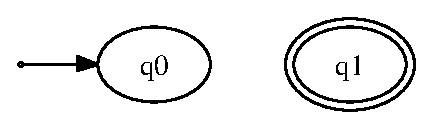
\epsfig{file=Abbildungen/aLeer.eps, scale=0.5}
      \caption{The \textsc{Fsm} $A(\emptyset)$.}
      \label{fig:aLeer.eps}
      \end{figure}
      Figure \ref{fig:aLeer.eps} shows the \textsc{Fsm} $A(\emptyset)$. It is obvious that we have
      $L\bigl(A(\emptyset)\bigr) = \{\}$. 
\item The \textsc{Fsm} $A(\varepsilon)$ is defined as
      \\[0.2cm]
      \hspace*{1.3cm}
      $A(\varepsilon) = \bigl\langle \{ q_0, q_1 \}, \Sigma, 
                          \bigl\{ \pair(q_0, \varepsilon) \mapsto \{q_1\} \bigr\}, q_0, \{ q_1 \} \bigr\rangle$.


      \begin{figure}[!ht]
        \centering
      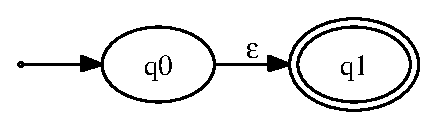
\epsfig{file=Abbildungen/aEpsilon.eps, scale=0.5}
      \caption{The \textsc{Fsm} $A(\varepsilon)$.}
      \label{fig:aEpsilon.eps}
      \end{figure}
      Figure \ref{fig:aEpsilon.eps} shows the \textsc{Fsm} $A(\varepsilon)$.
      We have that $L\bigl(A(\varepsilon)\bigr) = \{\texttt{''}\}$, i.e.~the \textsc{Fsm} only accepts the empty string. 
\item For a letter $c \in \Sigma$ the \textsc{Fsm} $A(c)$ is defined as 
      \\[0.2cm]
      \hspace*{1.3cm}
      $A(c) = \bigl\langle \{ q_0, q_1 \}, \Sigma, 
                                \bigl\{ \langle q_0, c \rangle \mapsto \{q_1\}\bigr\}, q_0, \{ q_1 \} \bigr\rangle$.

      \begin{figure}[!ht]
        \centering
      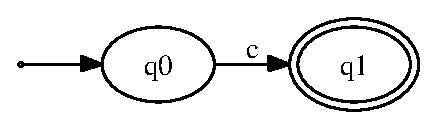
\epsfig{file=Abbildungen/aChar.eps, scale=0.5}
      \caption{The \textsc{Fsm} $A(c)$.}
      \label{fig:aChar.eps}
      \end{figure}
      Figure \ref{fig:aChar.eps} shows $A(c)$.
      We have that $L\bigl(A(c)\bigr) = \{c\}$, i.e.~the \textsc{Fsm} only accepts the character $c$. 
\item In order to define the \textsc{Fsm} $A(r_1 \cdot r_2)$ for the concatenation $r_1 \cdot r_2$ 
      we assume that the states in the \textsc{Fsm}s  $A(r_1)$ and $A(r_2)$ are different. 
      This can always be achieved by renaming the states of $A(r_2)$.
      Next, we assume that $A(r_1)$ and $A(r_2)$ have the following form:
      \begin{enumerate}
      \item $A(r_1) = \bigl\langle Q_1, \Sigma, \delta_1, q_1, \{ q_2 \}\bigr\rangle$,
      \item $A(r_2) = \bigl\langle Q_2, \Sigma, \delta_2, q_3, \{ q_4 \}\bigr\rangle$,
      \item $Q_1 \cap Q_2 = \{\}$.
      \end{enumerate}
      Then we can build the \textsc{Fsm} $A(r_1 \cdot r_2)$ from $A(r_1)$ and $A(r_2)$ as follows:
      \\[0.2cm]
      \hspace*{0.8cm}
       $A(r_1 \cdot r_2) := \bigl\langle Q_1 \cup Q_2, \Sigma, 
                \bigl\{ \pair(q_2,\varepsilon) \mapsto \{q_3\} \bigr\} 
                   \cup \delta_1 \cup \delta_2, q_1, \{ q_4 \} \bigr\rangle$
      \\[0.2cm]
      Here, the notation $\{ \pair(q_2,\varepsilon) \mapsto q_3 \} \cup \delta_1 \cup \delta_2$ specifies that
      $A(r_1 \cdot r_2)$ contains all transitions from both $A(r_1)$ and $A(r_2)$ and, furthermore,
      contains an $\varepsilon$-transition from $q_2$ to $q_3$.     
      Formally, this transition function  $\delta$ can be specified as follows:
      \\[0.2cm]
      \hspace*{1.3cm}
      $\delta(q,c) := \left\{
      \begin{array}{ll}
        \{ q_3 \}       & \mbox{if $q = q_2$ and $c = \varepsilon$}, \\[0.2cm]
        \delta_1(q, c)  & \mbox{if $q \in Q_1$ and $\pair(q,c) \not= \pair(q_2,\varepsilon)$}, \\[0.2cm]
        \delta_2(q, c)  & \mbox{if $q \in Q_2$.} 
      \end{array}\right.
      $
      \\[0.2cm]


      \begin{figure}[!ht]
        \centering
      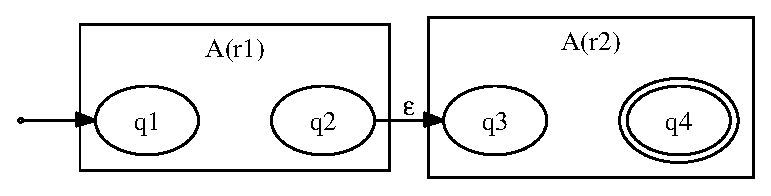
\epsfig{file=Abbildungen/aConcat.eps, scale=0.8}
      \caption{The \textsc{Fsm} $A(r_1 \cdot r_2)$.}
      \label{fig:aConcat.eps}
      \end{figure}
      Figure \ref{fig:aConcat.eps} shows the \textsc{Fsm} $A(r_1 \cdot r_2)$.

      Instead of having an $\varepsilon$-transition from $q_2$ to $q_3$ we can identify the states $q_2$ and
      $q_3$.  The advantage is that the resulting \textsc{Fsm} is smaller.
      We will do this when creating \textsc{Fsm}s by hand.  

      I haven't done this identification in the definition above because both the graphical representation and 
      the implementation get more complicated when we identify these states.
\item In order to define the \textsc{Fsm} $A(r_1 + r_2)$ we assume again that the states of the \textsc{Fsm}s
      $A(r_1)$ and $A(r_2)$ are different and that $A(r_1)$ and $A(r_2)$ have the following form:
      \begin{enumerate}
      \item $A(r_1) = \bigl\langle Q_1, \Sigma, \delta_1, q_1, \{ q_3 \}\bigr\rangle$,
      \item $A(r_2) = \bigl\langle Q_2, \Sigma, \delta_2, q_2, \{ q_4 \}\bigr\rangle$,
      \item $Q_1 \cap Q_2 = \{\}$.
      \end{enumerate}
      Then the \textsc{Fsm} $A(r_1 + r_2)$ is defined as follows:
      \\[0.2cm]
      \hspace*{0.8cm}
       $\bigl\langle \{ q_0, q_5 \} \cup Q_1 \cup Q_2, \Sigma, 
                \bigl\{ \pair(q_0,\varepsilon) \mapsto \{q_1, q_2\},
                   \pair(q_3,\varepsilon) \mapsto \{q_5\}, \pair(q_4,\varepsilon) \mapsto \{q_5\} \bigr\} 
                   \cup \delta_1 \cup \delta_2, q_0, \{ q_5 \} \bigr\rangle$

      \begin{figure}[!ht]
        \centering
      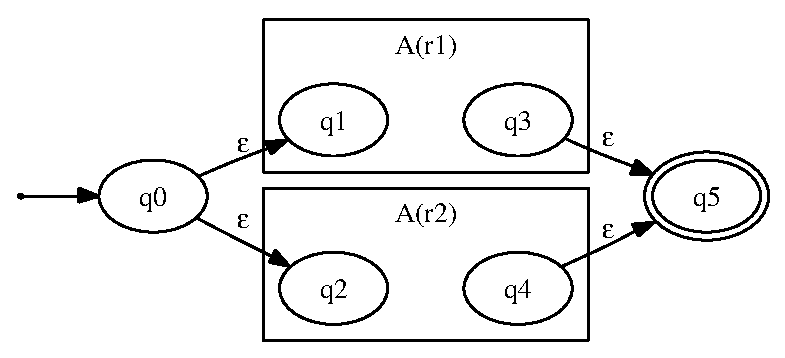
\epsfig{file=Abbildungen/aPlus.eps, scale=0.5}
      \caption{The \textsc{Fsm} $A(r_1 + r_2)$.}
      \label{fig:aPlus.eps}
      \end{figure}
      Figure \ref{fig:aPlus.eps} shows the \textsc{Fsm} $A(r_1 + r_2)$.
      In addition to the states of $A(r_1)$ and $A(r_2)$ there are two more states:
      \begin{enumerate}
      \item $q_0$ is the start state of the \textsc{Fsm} $A(r_1 + r_2)$,
      \item $q_5$ is the only accepting state of the \textsc{Fsm} $A(r_1 + r_2)$.
      \end{enumerate}
      In addition to the transitions of $A(r_1)$ and $A(r_2)$ the \textsc{Fsm} $A(r_1+r_2)$
      has four more $\varepsilon$-transitions.
      \begin{enumerate}
      \item The new start state $q_0$ has two
            $\varepsilon$-transitions leading to the start states $q_1$ and $q_2$ of the \textsc{Fsm}s
            $A(r_1)$ and $A(r_2)$.
      \item Each of the accepting states $q_3$ and $q_4$ of the \textsc{Fsm}s
             $A(r_1)$ and $A(r_2)$ has an $\varepsilon$-transition to the new accepting state $q_5$.
      \end{enumerate}
      In order to simplify this \textsc{Fsm} we could identify the three states
      $q_0$, $q_1$ and $q_2$ and the three states $q_3$, $q_4$ and $q_5$.  However, the resulting \textsc{Fsm}
      would be more difficult to understand and hence we are \underline{\red{not}} doing this when creating 
      \textsc{Fsm}s by hand.
\item In order to define the \textsc{Fsm} $A(r^*)$ we assume that
      \\[0.2cm]
      \hspace*{1.3cm}
      $A(r) = \bigl\langle Q, \Sigma, \delta, q_1, \{ q_2 \} \bigr\rangle$.
      \\[0.2cm]
      Then  $A(r^*)$ is defined as follows:
      \\[0.2cm]
      \hspace*{0.8cm}
       $\bigl\langle \{ q_0, q_3 \} \cup Q, \Sigma, 
                \bigl\{ \pair(q_0,\varepsilon) \mapsto \{q_1, q_3\}, \pair(q_2,\varepsilon) \mapsto \{q_1, q_3\} \bigr\} 
                \cup \delta, q_0, \{ q_3 \} \bigr\rangle$.
      \\[0.2cm]


      \begin{figure}[!ht]
        \centering
      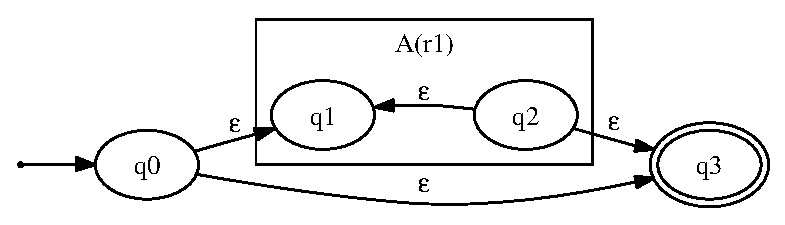
\epsfig{file=Abbildungen/aStar.eps, scale=0.5}
      \caption{The \textsc{Fsm} $A(r^*)$.}
      \label{fig:aStar.eps}
      \end{figure}
      Figure \ref{fig:aStar.eps} shows the \textsc{Fsm} $A(r^*)$.
      In comparison with $A(r)$ this \textsc{Fsm} has two additional states.
      \begin{enumerate}
      \item $q_0$ is the start state of $A(r^*)$,
      \item $q_3$ is the only accepting state of $A(r^*)$.
      \end{enumerate}
      The \textsc{Fsm} $A(r^*)$ has four more $\varepsilon$-transitions than $A(r)$: 
      \begin{enumerate}
      \item The new start state  $q_0$ has $\varepsilon$-transitions to the states
            $q_1$ and $q_3$.
      \item $q_2$ has an $\varepsilon$-transition back to the state $q_1$.
      \item $q_2$ also has an $\varepsilon$-transition to the state $q_3$.
      \end{enumerate}
      \textbf{\textcolor{red}{Attention}}:  If we would identify the two states 
      $q_0$ and $q_1$ and the two states $q_2$ and $q_3$, then the resulting \textsc{Fsm} would no longer be
      correct!
\end{enumerate}

\exerciseEng
Construct a non-deterministic \textsc{Fsm} that accepts the language specified by the regular expression
\\[0.2cm]
\hspace*{1.3cm}
$\texttt{a}^* \cdot \texttt{b}^*$.
\\[0.2cm]
Consider what would happen if you would identify the two states 
$q_0$ and $q_1$ and the two states $q_2$ and $q_3$ in step 6 of the construction given above. 
\eox

\exerciseEng
Construct a non-deterministic \textsc{Fsm} for the regular expression
\\[0.2cm]
\hspace*{1.3cm}
$(\texttt{a} + \texttt{b}) \cdot \texttt{a}^* \cdot \texttt{b}$.  
\eox

\subsection{Implementation}
The \textsl{Jupyter notebook}
\href{https://github.com/karlstroetmann/Formal-Languages/blob/master/Python/Regexp-2-NFA.ipynb}{Regexp-2-NFA.ipynb} 
implements the theory discussed in this section.



\section{Translating a Deterministic \textsc{Fsm} into a Regular Expression}
In this last section we start with a deterministic \textsc{Fsm} $F$ and construct a regular expression $r$
such that we have
\\[0.2cm]
\hspace*{1.3cm}
$L(r) = L(F)$. 
\\[0.2cm]
We assume that the \textsc{Fsm} $F$ is given as follows:
\\[0.2cm]
\hspace*{1.3cm}
$F = \bigl\langle \{ q_0, q_1, \cdots, q_n \}, \Sigma, \delta, q_0, A \bigr\rangle$.
\\[0.2cm]
For every pair of states $\pair(p_1,p_2) \in Q \times Q$ we define a regular expression
$r(p_1, p_2)$ such that $r(p_1, p_2)$ describes those strings $w$ that take the \textsc{Fsm} $F$ from the state
$p_1$ to the state $p_2$, i.e.~we have
\\[0.2cm]
\hspace*{1.3cm}
$L\bigl(r(p_1, p_2)\bigr) = 
  \bigl\{ w \in \Sigma^* \mid \pair(p_1,w) \leadsto^* \pair(p_2, \varepsilon) \bigr\}$.
\\[0.2cm]  
The definition of $r(p_1, p_2)$ is done by first defining auxiliary regular expressions 
$r^{(k)}(p_1, p_2)$ for all $k =0,\cdots,n+1$.   The regular expression $r^{(k)}(p_1, p_2)$ specifies those
strings that take the \textsc{Fsm} $F$ from the state
$p_1$ to the state $p_2$ without visiting a state from the set
\\[0.2cm]
\hspace*{1.3cm}
$Q_k := \bigl\{ q_i \mid i \in \{k,\cdots,n \}  \bigl\} = \{ q_k, \cdots, q_n \}$.
\\[0.2cm]
To this end we define the ternary relation
\\[0.2cm]
\hspace*{1.3cm}
$\mapsto_k \;\subseteq\; (Q \times \Sigma^* \times Q)$.
\\[0.2cm]
Given two states $p, q \in Q$ and a string $w$ we have that
\\[0.2cm]
\hspace*{1.3cm}
$p \stackrel{w}{\mapsto}_k q$
\\[0.2cm]
holds iff the \textsc{Fsm} $F$ switches from the state $p$ to the state $q$ when it reads the string $w$
but on reading $w$ does not switch to a state from the set
$Q_k$ \blue{in-between}.  Here, ``in-between'' specifies that the states $p$ and $q$ may well be elements of the set
$Q_k$, only the states between $p$ and $q$ must not be in $Q_k$.
The formal definition of $p \stackrel{w}{\mapsto}_k q$ is done by induction on  $w$:
\begin{enumerate}
\item[B.C.:] $|w| \leq 1$.  Then there are two cases:
  \begin{enumerate}
  \item $p \stackrel{\varepsilon}{\mapsto}_k p$,

        because when the empty string is read we can only reach the state $p$ if we start in the state $p$.
  \item $\delta(p, c) = q \;\Rightarrow\; p \stackrel{c}{\mapsto}_k q$,

        because when the \textsc{Fsm} reads the character $c$ and switches from state $p$ directly
        to the state $q$, there are no states ``inbetween''.
  \end{enumerate}
\item[I.S.:] $w = cv$ where $|v| \geq 1$.

             Here we have:
             \hspace*{1.3cm}
            $p \stackrel{c}{\mapsto} q \wedge q \not\in Q_k \wedge q \stackrel{v}{\mapsto}_k r
              \Rightarrow p \stackrel{cv}{\mapsto}_k r$.
\end{enumerate}
Now we are ready to define the regular expressions $r^{(k)}(p_1, p_2)$ for all $k=0,\cdots,n+1$.
This definition will be done such that we have
\\[0.2cm]
\hspace*{1.3cm}
$L\bigl(r^{(k)}(p_1, p_2)\bigr) = \bigl\{ w \in \Sigma^* \mid p_1 \stackrel{w}{\mapsto}_k p_2 \bigr\}$.
\\[0.2cm]
The definition of the regular expressions $r^{(k)}(p_1, p_2)$ is done by induction on $k$.
\begin{enumerate}
\item[B.C.:] $k = 0$.  

  Then we have $Q_0 = Q$ and therefore the set $Q_0$ contains all states.
  Therefore, when the \textsc{Fsm} switches from the state $p_1$ to the state $p_2$ it must not visit any
  states in-between.  There are two cases.
  \begin{enumerate}
  \item $p_1 \not= p_2$:  Then we can have  $p_1 \stackrel{w}{\mapsto}_0 p_2$ only if $w$ contains but a
        single letter.  Define
        \\[0.2cm]
        \hspace*{1.3cm}
        $\{ c_1, \cdots, c_l \} := \{ c \in \Sigma \mid \delta(p_1,c) = p_2 \}$
        \\[0.2cm]
        as the set of all letters that take the \textsc{Fsm} from the state $p_1$ to the state $p_2$.
        If this set is not empty we define 
        \\[0.2cm]
        \hspace*{1.3cm}
        $r^{(0)}(p_1, p_2) := c_1 + \cdots + c_l$. 
        \\[0.2cm]
        If this set is empty, then there is no direct transition from  $p_1$ to $p_2$ and we define
        \\[0.2cm]
        \hspace*{1.3cm}
        $r^{(0)}(p_1, p_2) := \emptyset$.
  \item $p_1 = p_2$:  Again we define
        \\[0.2cm]
        \hspace*{1.3cm}
        $\{ c_1, \cdots, c_l \} := \{ c \in \Sigma \mid \delta(p_1,c) = p_1 \}$.
        \\[0.2cm]
        If this set is not empty we have
        \\[0.2cm]
        \hspace*{1.3cm}
        $r^{(0)}(p_1, p_1) := c_1 + \cdots + c_l + \varepsilon$.
        \\[0.2cm]
        Otherwise we have
        \\[0.2cm]
        \hspace*{1.3cm}
        $r^{(0)}(p_1, p_1) := \varepsilon$.
   \end{enumerate}
\item[I.S.:] $k \mapsto k+1$.  

  When compared to the regular expression $r^{(k)}(p_1, p_2)$,
  the regular expression  $r^{(k+1)}(p_1, p_2)$ is allowed to use the state
  $q_k$, because $q_k$ is the only element of the set $Q_k$ that is not a member of the set $Q_{k+1}$.  
  If the \textsc{Fsm} reads a string $w$ that switches the state $p_1$ to the state $p_2$ without switching into a state
  from the set $Q_{k+1}$, then there are two cases.
  \begin{enumerate}
  \item We already have $p_1 \stackrel{w}{\mapsto}_k p_2$.
  \item The string $w$ can be written as  $w = w_1 s_1\cdots s_l w_2$ where we have:
        \begin{itemize}
        \item $p_1 \stackrel{w_1}{\mapsto}_k q_k$,
        \item $q_k \stackrel{s_i}{\mapsto}_k q_k$ \quad for all $i = \{ 1, \cdots, l\}$,
        \item $q_k \stackrel{w_2}{\mapsto}_k p_2$.
        \end{itemize}
        Therefore we define
        \\[0.2cm]
        \hspace*{1.3cm}
        $r^{(k+1)}(p_1,p_2) := 
         r^{(k)}(p_1,p_2) + 
         r^{(k)}(p_1,q_k) \cdot \bigl(r^{(k)}(q_k,q_k)\bigr)^* \cdot r^{(k)}(q_k,p_2)$.
  \end{enumerate}  
\end{enumerate}
Now we are ready to define the regular expressions $r(p_1,p_2)$ for all states $p_1$ and $p_2$:
\\[0.2cm]
\hspace*{1.3cm}
$r(p_1,p_2) := r^{(n+1)}(p_1,p_2)$. 
\\[0.2cm]
This regular expression specifies all strings that take the \textsc{Fsm} from the state
$p_1$ to the state $p_2$ without using any state from the set 
$Q_{n+1}$ in-between.   Since we have
\\[0.2cm]
\hspace*{1.3cm}
$Q_{n+1} = \bigl\{ q_i \mid i \in \{0,\cdots,n \} \wedge i \geq n+1 \bigr\} = \{\}$
\\[0.2cm]
we know that $Q_{n+1}$ is empty.
Therefore the regular expression $r^{(n+1)}(p_1,p_2)$
does not exclude any states when switching from
state $p_1$ to the state $p_2$.

In order to construct a regular expression that specifies the language accepted by a deterministic \textsc{Fsm}
$F$ we write the set $A$ of accepting states of $F$ as
\\[0.2cm]
\hspace*{1.3cm}
$A = \{ t_1, \cdots, t_m \}$.
\\[0.2cm]
Then the regular expression $r(A)$ is defined as
\\[0.2cm]
\hspace*{1.3cm}
$r(A) := r(q_0, t_1) + \cdots + r(q_0, t_m)$.
\\[0.2cm]
This regular expression specifies those strings that take the \textsc{Fsm} $F$ from its start state $q_0$ into
any of its accepting states.
\qed


\exerciseEng
Take the \textsc{Fsm} shown in Figure \ref{fig:abstara.dot} and construct an equivalent regular expression.


\solutionEng
The \textsc{Fsm} has two states: $0$ and $1$.  We start by computing the regular expressions
$r^{(k)}(i,j)$ for all $i,j\in\{0,1\}$ for  $k =0$, $1$ und $2$:
\begin{enumerate}
\item For $k = 0$ we have:
      \begin{enumerate}
      \item $r^{(0)}(0, 0) = \texttt{a} + \varepsilon$,
      \item $r^{(0)}(0, 1) = \texttt{b}$,
      \item $r^{(0)}(1, 0) = \emptyset$,
      \item $r^{(0)}(1, 1) = \texttt{a} + \varepsilon$.
      \end{enumerate}
\item For $k=1$ we have:
      \begin{enumerate}
      \item For $r^{(1)}(0, 0)$ we have:
            \begin{eqnarray*}
                  r^{(1)}(0, 0) 
            & = & r^{(0)}(0, 0) + 
                  r^{(0)}(0, 0) \cdot \bigl(r^{(0)}(0, 0)\bigr)^* \cdot r^{(0)}(0, 0) \\
            & \doteq & r^{(0)}(0, 0) \cdot \bigl(r^{(0)}(0, 0)\bigr)^*
            \end{eqnarray*}
             In the last step we used the fact that 
             \\[0.2cm]
             \hspace*{1.3cm}
             $
             \begin{array}[t]{lcl}
               r + r \cdot r^* \cdot r & \doteq & r \cdot (\varepsilon + r^* \cdot r) \\
                                       & \doteq & r \cdot r^*
             \end{array}
             $
             \\[0.2cm]
             to simplify the result.
             If we substitute for $r^{(0)}(0, 0)$ the expression $\texttt{a} + \varepsilon$  
             we get 
             \\[0.2cm]
             \hspace*{1.3cm}
             $r^{(1)}(0, 0) \doteq (\texttt{a} + \varepsilon)\cdot (\texttt{a} + \varepsilon)^*$.
             \\[0.2cm]
             As we have $(\texttt{a} + \varepsilon)\cdot (\texttt{a} + \varepsilon)^* \doteq \texttt{a}^*$ we have
             \\[0.2cm]
             \hspace*{1.3cm}
             $r^{(1)}(0, 0) \doteq \texttt{a}^*$.
      \item For $r^{(1)}(0, 1)$ we have:
            \begin{eqnarray*}
                  r^{(1)}(0, 1) 
            & \doteq & r^{(0)}(0, 1) + 
                  r^{(0)}(0, 0) \cdot \bigl(r^{(0)}(0, 0)\bigr)^* \cdot r^{(0)}(0, 1) \\
            & \doteq & \texttt{b} + 
                  (\texttt{a} + \varepsilon) \cdot (\texttt{a} + \varepsilon)^* \cdot \texttt{b} \\
            & \doteq & \texttt{b} + \texttt{a}^* \cdot \texttt{b} \\
            & \doteq & (\varepsilon + \texttt{a}^*) \cdot \texttt{b} \\
            & \doteq & \texttt{a}^* \cdot \texttt{b} 
        \end{eqnarray*}
      \item For $r^{(1)}(1, 0)$ we have:
            \begin{eqnarray*}
                  r^{(1)}(1, 0) 
            & \doteq & r^{(0)}(1, 0) + 
                  r^{(0)}(1, 0) \cdot \bigl(r^{(0)}(0, 0)\bigr)^* \cdot r^{(0)}(0, 0) \\
            & \doteq & \emptyset + \emptyset \cdot (\texttt{a} + \varepsilon)^* \cdot (\texttt{a} + \varepsilon) \\
            & \doteq & \emptyset
            \end{eqnarray*}
      \item For $r^{(1)}(1, 1)$ we have
            \begin{eqnarray*}
                  r^{(1)}(1, 1)
            & \doteq & r^{(0)}(1, 1) + 
                  r^{(0)}(1, 0) \cdot \bigl(r^{(0)}(0, 0)\bigr)^* \cdot r^{(0)}(0, 1) \\
            & \doteq & (\texttt{a} + \varepsilon) + 
                  \emptyset \cdot (\texttt{a} + \varepsilon)^* \cdot \texttt{b} \\
            & \doteq & (\texttt{a} + \varepsilon) + \emptyset  \\
            & \doteq & \texttt{a} + \varepsilon  
            \end{eqnarray*}
      \end{enumerate}
\item For $k=2$ we only have to compute the regular expression $r^{(2)}(0, 1)$:
            \begin{eqnarray*}
                  r^{(2)}(0, 1)
            & \doteq & r^{(1)}(0, 1) + 
                  r^{(1)}(0, 1) \cdot \bigl(r^{(1)}(1, 1)\bigr)^* \cdot r^{(1)}(1, 1) \\
            & \doteq & \texttt{a}^* \cdot \texttt{b} + 
                  \texttt{a}^* \cdot \texttt{b} \cdot (\texttt{a} + \varepsilon)^* \cdot (\texttt{a} + \varepsilon) \\
            & \doteq & \texttt{a}^* \cdot \texttt{b} + \texttt{a}^* \cdot \texttt{b} \cdot \texttt{a}^* \\
            & \doteq & \texttt{a}^* \cdot \texttt{b} \cdot (\varepsilon + \texttt{a}^*) \\
            & \doteq & \texttt{a}^* \cdot \texttt{b} \cdot \texttt{a}^*.
        \end{eqnarray*}
\end{enumerate}
As the state 0 is the start state and the state $1$ is the only accepting state we have
\\[0.2cm]
\hspace*{1.3cm}
$r(F) = r^{(2)}(0, 1) \doteq \texttt{a}^* \cdot \texttt{b} \cdot \texttt{a}^*$.
\\[0.2cm]
\qed

\exerciseEng
Take the \textsc{Fsm} shown in Figure \ref{fig:exercise-13.eps} on page
\pageref{fig:exercise-13.eps} and construct a regular expression specifying the same language as this
\textsc{Fsm}.

\begin{figure}[!ht]
  \centering
\epsfig{file=Abbildungen/exercise-13.eps, scale=1.0}
\caption{A deterministic finite state machine.}
\label{fig:exercise-13.eps}
\end{figure}

\subsection{Implementation}
The \textsl{Jupyter notebook} 
\\[0.2cm]
\hspace*{1.3cm}
\href{https://github.com/karlstroetmann/Formal-Languages/blob/master/Python/DFA-2-RegExp.ipynb}{https://github.com/karlstroetmann/Formal-Languages/blob/master/Python/DFA-2-RegExp.ipynb}
\\[0.2cm]
contains a program that takes a deterministic \textsc{Fsm} $F$ and computes a regular expression $r$ such that
$r$ specifies the language accepted by $F$, i.e.~we have $L(r) = L(F)$.

\section{Minimization of Finite State Machines}
In this section we show how to minimize the number of states of a deterministic finite state machine
\\[0.2cm]
\hspace*{1.3cm}
$F = \langle Q, \Sigma, \delta, q_0, A \rangle$.
\\[0.2cm]
Without loss of generality we want to assume that the \textsc{Fsm} $F$ is complete: Therefore, we assume that
for each state $q \in Q$ and each letter $c \in \Sigma$ the expression $\delta(q, c)$ 
returns a state of $Q$.  Our goal is to find a deterministic finite state machine
\\[0.2cm]
\hspace*{1.3cm}
$F^- = \langle Q^-, \Sigma, \delta^-, q_0, A^- \rangle$,
\\[0.2cm]
which accepts the same language as  $F$, so 
\\[0.2cm]
\hspace*{1.3cm}
$L(F^-) = L(F)$
\\[0.2cm]
and for which the number of states of the set $Q^-$ is minimal.  
We start with the function 
\\[0.2cm]
\hspace*{1.3cm}
$\delta^*: Q \times \Sigma^* \rightarrow Q$
\\[0.2cm]
which extends the function $\delta$ by accepting a string instead of a single character as its first argument.
The function call $\delta^*(q,s)$ calculates the state $p$ which the \textsc{Fsm} $F$ enters if it reads the
string $s$ in the state $q$. As we have assumed the \textsl{Fsm} F to be complete, we have that
\\[0.2cm]
\hspace*{1.3cm}
$\delta(q, c) \not\in \Omega$ \quad for all $q \in Q$ and all $c \in \Sigma$ 
\\[0.2cm]
and then $\delta^*(q,w)$ is defined by induction on $w$ as follows:
\begin{enumerate}[(a)]
\item $\delta^*(q, \varepsilon) := q$ \quad for all $q \in Q$.
\item $\delta^*(q, cw) := \delta^*(\delta(q, c), v)$ \quad for all $q \in Q$, $c \in \Sigma$, and $v \in \Sigma^*$.
\end{enumerate}
Since the function $\delta^*$ is a generalization of the function $\delta$, in
the future we will not distinguish in the notation between $\delta$ and $\delta^*$ and write $\delta$ for both functions. 

Obviously, in a finite state machine 
$F = \langle Q, \Sigma, \delta, q_0, A \rangle$ we can remove all the states $p \in Q$ which are not
\blue{reachable} from the start state.  A state $p$ is \blue{reachable}\index{reachable} iff 
a string $w \in \Sigma^*$ is given, such that
\\[0.2cm]
\hspace*{1.3cm}
$\delta(q_0, w) = p$
\\[0.2cm]
holds.  In the following we assume that all states of the \textsc{Fsm} $F$ can be reached
from the start state. 


\begin{figure}[!ht]
  \centering
  \epsfig{file=Abbildungen/nicht-gleichwertig.eps, scale=0.6}
   \caption{A finite state machine with equivalent states.}
  \label{fig:nicht-gleichwertig.dot}
\end{figure}

In general, we can minimize an \textsc{Fsm} by identifying certain states.   
If we look for example at the \textsc{Fsm} shown in figure \ref{fig:nicht-gleichwertig.dot}, we can identify
the states $q_1$ and $q_2$ as well as $q_3$ and $q_4$ without changing the language of the \textsc{Fsm}. 
The central idea in minimizing a \textsc{Fsm} is that we compute those states which \textbf{must not} be
identified and consider all other states as equivalent.  States that must not be identified are called
\blue{separable states}.  This notion is defined next.

\begin{Definition}[Separable States]
Assume $F = \langle Q, \Sigma, \delta, q_0, A \rangle$ is a deterministic finite state machine.
Two states $p_1,p_2 \in Q$ are called \blue{separable} \index{separable} if and only if there exists a string 
$s \in \Sigma^*$ such that either
\begin{enumerate}
\item $\delta(p_1,s) \in    A$ and $\delta(p_2,s) \notin A$ or
\item $\delta(p_1,s) \notin A$ and $\delta(p_2,s) \in    A$
\end{enumerate}
holds.  In this case, the string $s$ \blue{separates} \index{separates} $p_1$ and $p_2$. \qed
\end{Definition}
If two states $p_1$ and $p_2$ are separable, then it is obvious that theses states must not be identified.
We define an equivalence relation $\sim$ on the set $Q$ of all states by setting
\\[0.2cm]
\hspace*{1.3cm}
$p_1 \sim p_2$ \quad iff \quad 
$\forall s \in \Sigma^*:\bigl(\delta(p_1,s) \in A \leftrightarrow \delta(p_2,s) \in A\bigr)$.
\\[0.2cm]
Hence, two states $p_1$ and $p_2$ are considered to be equivalent iff they are not separable.   
The claim is that we can identify all pairs $\langle p_1, p_2\rangle$ of equivalent states.  The
\blue{identification} \index{identification of states} 
of two states $p_1$ and $p_2$ is done by removing the state $p_2$ from the set $Q$ and changing the transition
function $\delta$ in a way that the new version of $\delta$ will return $p_1$ in all those cases where the old
version of $\delta$ had returned $p_2$. 


The question remains how we can determine which states are distinguishable.
One possibility is to create a set $V$ with pairs of states.  We add the pair $\langle p, q \rangle$ to the set
$V$ if we have discovered that $p$ and $q$ are distinguishable.  We recognize $p$ and $q$ as distinguishable if
there is a letter $c\in\Sigma$ and two states $s$ and $t$ that are already known to be distinguishable such that 
\\[0.2cm]
\hspace*{1.3cm}
$\delta(p,c) = s$, \quad $\delta(q,c) = t$, \quad and \quad $\langle s, t \rangle \in V$
\\[0.2cm]
holds. This idea leads to an algorithm that uses two steps:
\begin{enumerate}[(a)]
\item First we initialize $V$ with all the pairs $\pair(p,q)$, for which either $p$ is an accepting state and
      $q$ is not an accepting state, or $q$ is an accepting state and $p$ is not an accepting state,
      because an accepting state can be distinguished from a non-accepting state by the empty string
      $\varepsilon$: 
      \\[0.2cm]
      \hspace*{1.3cm}
      $V := \bigl\{\pair(p,q) \in Q \times Q \mid (p \in A \wedge q \notin A) \vee 
      (p \notin A \wedge q \in A) \bigr\}$
      \\[0.2cm]
      This can also be written as the union of two Cartesian products. We have
      \\[0.2cm]
      \hspace*{1.3cm}
      $V = A \times (Q \backslash A) \cup (Q \backslash A) \times A$.
\item As long as we find a new pair $\pair(p,q) \in Q \times Q$ for which there is a letter $c$ such that the
      states $\delta(p,c)$ and $\delta(q,c)$ are already distinguishable, we add this pair to the set $V$:  
      \\[0.2cm]
      \hspace*{1.3cm} 
      \texttt{while $\exists \pair(p,q) \in Q \times Q: \exists c \in \Sigma:\langle\delta(p,c),
        \delta(q,c)\rangle \in V \wedge \pair(p,q) \notin V$ } \\
      \hspace*{1.8cm}
      \texttt{choose $\pair(p,q) \in Q \times Q$ such that} $\langle\delta(p,c),
      \delta(q,c)\rangle \in V \wedge \pair(p,q) \notin V$ \\
      \hspace*{2.3cm}
      \texttt{$V$ := $V \cup \{\, \pair(p,q),\, \pair(q,p)\, \}$;} \\
\end{enumerate}
If we have found all pairs $\pair(p,q)$ of distinguishable states, then we can identify all states $p$ and $q$
which are not distinguishable and therefore $\langle p, q \rangle \not\in V$.   The \textsc{Fsm} constructed in
this way is, in fact, minimal.  

\exerciseEng
We consider the  \textsc{Fsm} shown in figure \ref{fig:nicht-gleichwertig.dot} and apply the algorithm
described above to this \textsc{Fsm}. 
We use a table for this.  The columns and rows of this table are numbered with the different states.  If we
have recognized in the first step that the states $i$ and $j$ are distinguishable, we insert a $1$ in this
table in the $i$-th row and the $j$-th column. 
Furthermore, since the states $i$ and $j$ can also be distinguished from the states $j$ and $i$, we also insert
a $1$ in the $j$-th row and the $i$-th column. 
\begin{enumerate}
\item In the first step we recognize that the two accepting states $q_3$ and $q_4$ are distinguishable from all non-accepting states.
      So the pairs 
      $\pair(q_0,q_3)$,
      $\pair(q_0,q_4)$,
      $\pair(q_1,q_3)$,
      $\pair(q_1,q_4)$,
      $\pair(q_2,q_3)$ and
      $\pair(q_2,q_4)$
      are distinguishable. So the table now has the following configuration:
      \begin{center}        
      \begin{tabular}[t]{|l||l|l|l|l|l|}
      \hline
            & $q_0$    &    $q_1$ &    $q_2$ &      $q_3$ &      $q_4$  \\
      \hline
      \hline
      $q_0$ &          &          &          & $1$ & $1$  \\
      \hline
      $q_1$ &          &          &          &$1$ &$1$  \\
      \hline
      $q_2$ &          &          &          &$1$ &$1$  \\
      \hline
      $q_3$ &$1$        &$1$         &       $1$ &          &           \\
      \hline
      $q_4$ &$1$ &$1$ &$1$ &          &           \\
      \hline
      \end{tabular}
      \end{center}
\item Next we see that the states $q_0$ and $q_1$ are distinguishable because
      \\[0.2cm]
      \hspace*{1.3cm}
      $\delta(q_0,a) = q_1$, \quad $\delta(q_1,a) = q_3$ \quad and \quad $q_1 \not\sim q_3$.
      \\[0.2cm]
      Also we see that the states $q_0$ and $q_2$ are distinguishable, because
      \\[0.2cm]
      \hspace*{1.3cm}
      $\delta(q_0,b) = q_2$, \quad $\delta(q_2,b) = q_4$ \quad and \quad $q_2 \not\sim q_4$.
      \\[0.2cm]
      Since we have found in the second step that $q_0 \not\sim q_1$ and $q_0 \not\sim q_2$ holds true, we will insert a $2$ at the corresponding positions in the table. Therefore the table now has the following form:
      \begin{center}        
      \begin{tabular}[t]{|l||l|l|l|l|l|}
      \hline
        & $q_0$      &      $q_1$ &      $q_2$ &      $q_3$ &      $q_4$  \\
      \hline
      \hline
      $q_0$ &          &$2$ &$2$ &$1$ &$1$  \\
      \hline
      $q_1$ &$2$ &          &          &$1$ &$1$  \\
      \hline
      $q_2$ &$2$ &          &          &$1$ &$1$  \\
      \hline
      $q_3$ &$1$ &$1$ &$1$ &          &           \\
      \hline
      $q_4$ &$1$ &$1$ &$1$ &          &           \\
      \hline
      \end{tabular}
      \end{center}
\item Now we do not find any more pairs of distinguishable states, because if we take a look at the pair $\pair(q_1,q_2)$ we can see that
      \\[0.2cm]
      \hspace*{1.3cm}
      $\delta(q_1,\texttt{a}) = q_3$ \quad and \quad $\delta(q_2,\texttt{a}) = q_4$, 
      \\[0.2cm]
      but because the states $q_3$ and $q_4$ are not distinguishable so far, this does not yield a new
      distinguishable pair.  Neither does 
      \\[0.2cm]
      \hspace*{1.3cm}
      $\delta(q_1,\texttt{b}) = q_3$ \quad and \quad $\delta(q_2,\texttt{b}) = q_4$
      \\[0.2cm]
      yield a new distinguishable pair.  At this point, the two states $q_3$ and $q_4$ remain.  We find
      \\[0.2cm]
      \hspace*{1.3cm}
      $\delta(q_3,c) = q_1$ \quad and \quad $\delta(q_4,c) = q_2$ \quad for all $c \in \{\texttt{a}, \texttt{b}\}$
      \\[0.2cm]
      and because the states $q_1$ and $q_2$ are not yet known to be distinguishable, we have not found any new distinguishable states.
      So we can read the equivalent states from the table, it holds that:
      \begin{enumerate}
      \item $q_1 \sim q_2$
      \item $q_3 \sim q_4$
      \end{enumerate}
      Figure \ref{fig:gleichwertig.dot} shows the corresponding reduced finite \textsc{Fsm}.
\end{enumerate}


\begin{figure}[!ht]
  \centering
  \epsfig{file=Abbildungen/gleichwertig.eps, scale=0.6}
   \caption{The reduced \textsc{Fsm}.}
  \label{fig:gleichwertig.dot}
\end{figure}



\exerciseEng
Construct the minimal deterministic  \textsc{Fsm} that recognizes the language 
$L\bigl(a \cdot (b \cdot a)^*\bigr)$.  Perform the following steps:
\begin{enumerate}[(a)]
\item Construct a non-deterministic \textsc{Fsm} which recognizes this language.
\item Transform this non-deterministic \textsc{Fsm} into a deterministic \textsc{Fsm}.
\item Minimize the number of states of this \textsc{Fsm} with the algorithm given above.
\end{enumerate}

\subsection{Implementation}
The \textsl{Jupyter notebook} 
\\[0.2cm]
\hspace*{1.3cm}
\href{https://github.com/karlstroetmann/Formal-Languages/blob/master/Python/DFA-2-RegExp.ipynb}{https://github.com/karlstroetmann/Formal-Languages/blob/master/Python/Minimize.ipynb}
\\[0.2cm]
contains a program that takes a deterministic \textsc{Fsm} $F$ and returns an equivalent \textsc{Fsm} that has
the minimum number of states.


\section{Conclusion}
In this chapter we have shown that the concept of a \blue{deterministic finite state machine}
and a \blue{regular expression} are equivalent.
\begin{enumerate}[(a)]
\item Every deterministic finite state machine can be translated into an equivalent regular expression.
\item Every regular expression can be translated into an equivalent non-deterministic \textsc{Fsm}.
\item Every non-deterministic \textsc{Fsm} can be transformed into an equivalent
      deterministic \textsc{Fsm}.
\end{enumerate}
Furthermore, we have shown that every deterministic finite state machine can be minimized.

\paragraph{Historical Remark}
\href{http://en.wikipedia.org/wiki/Stephen_Cole_Kleene}{Stephen C.~Kleene} (1909 -- 1994) has shown in 1956 that the concepts of 
\blue{finite state  machines} and \blue{regular expression} have the same strength
\cite{kleene:1956}.


\section{Check your Understanding}
\begin{enumerate}[(a)]
\item How are deterministic and non-deterministic finite state machines defined?
\item Given a non-deterministic \textsc{Fsm} $F$, can you convert it into a deterministic \textsc{Fsm}
      $\mathtt{det}(F)$ that accepts the same language as the \textsc{Fsm} $F$?
\item Given a regular expression $r$, can you describe the steps necessary to construct a non-deterministic
      \textsc{Fsm} $F$ that accepts the language specified by $r$?
\item Given a deterministic \textsc{Fsm} $F$ can you describe how to construct a regular expression $r$
      that specifies the language accepted by $F$?
\item How do we mimimize a finite state machine?
\end{enumerate}

%%% Local Variables: 
%%% mode: latex
%%% TeX-master: "formal-languages.tex"
%%% End: 
